\documentclass{article}
\usepackage{geometry}[margin=1cm]
\usepackage{graphicx}
\usepackage{amssymb}
\begin{document}

{\bf Solution to Problem 1}

Let $OK$ be the height from $O$ to $AB$. As the segment $AB$ is a chord of $\Gamma$, $K$ is the midpoint of the segment $AB$.
$\sphericalangle BAB'$ is a right angle because it subtends the diagonal of $\Gamma$. 
Let $O'$ be the height from $O'$ to $AB$. As $O'K'$ is parallel to $OK$ and to $AB'$ and $|OO'|=|O'B'|$ it follows that $|K'K|=|AK'|$. As the height from the centre of a circle to its chord divides the chord at its midpoint, it follows that $K$ is on $\Gamma'$.

\begin{center}
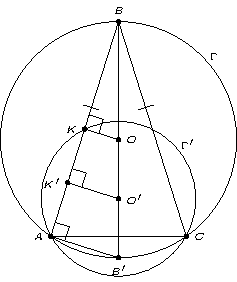
\includegraphics[width=0.5\textwidth]{Figures/fig2}
\end {center}

\end{document}
